\documentclass[12pt]{article}
\usepackage[utf8]{inputenc}
\usepackage[margin=1in]{geometry}
\usepackage{hyperref,indentfirst,amstext,amsmath,amssymb,amsthm,esint,float,graphicx,caption,array,wrapfig}
\usepackage{mathtools}

\usepackage[hyperref=true,backref=true,sorting=none]{biblatex}
\hypersetup{colorlinks=true,linkcolor=red,citecolor=red,urlcolor=blue}
\addbibresource{main.bib}
\renewcommand*{\bibfont}{\small}

\let\Pr\relax
\DeclareMathOperator*{\Pr}{\mathbb{P}}
\DeclareMathOperator*{\E}{\mathbb{E}}
\graphicspath{{./graphs/}}
\newcolumntype{P}[1]{>{\centering\arraybackslash}p{#1}}
\newcolumntype{M}[1]{>{\centering\arraybackslash}m{#1}}
\newcommand\scalemath[2]{\scalebox{#1}{\mbox{\ensuremath{\displaystyle #2}}}}
\renewcommand\arraystretch{1.5}

\DeclarePairedDelimiter\floor{\lfloor}{\rfloor}

\parindent 0.3in
\title{A Survey of Multi-Armed Bandit Learning}
\author{James Heppenstall, Haochen Li, Alberto Mizrahi}
\date{7 May 2019}

\begin{document}
\maketitle

\section{Introduction}

In this project, we focus on two formalizations of the multi-armed bandit problem: \textbf{stochastic i.i.d rewards} and \textbf{adversarial rewards}. For the former, we survey epsilon strategies, UCB strategies, and Thompson sampling. For the latter, we survey the Exp3 and Exp3.P algorithms. In particular, we experimentally verify their regret bounds and compare their performance on Bernouilli trials and adversarial data. We finally motivate the problem in the broader context of Princeton's Theoretical Machine Learning (COS 511) course.

At a high level, the multi-armed bandit problem is a sequential decision problem concerned with how one dynamically allocates a resource among a set of actions to maximize some cumulative reward \cite{robbins1952}. While the original motivation for this problem came from clinical trials \cite{thompson1933}, the term ``multi-armed bandit" actually traces back to slot machines, each colloquially referred to as a ``one-armed bandit", by virtue of the arm one pulls down and the fact that they often empty gamblers' pockets. It should come as no surprise that Gittins' canonical example therefore considers a gambler who must decide which arm to pull among $K$ non-identical slot machines in order to maximize his return \cite{gittins1979}.

The multi-armed bandit learning problem has received much attention, particularly in the reinforcement learning community, because it touches upon the intrinsic tradeoff between \textbf{exploration} and \textbf{exploitation} in sequential experiments \cite{bubeck2012}. In the context of Gittins' slot machines, should one \textit{explore} slot machines with unknown rewards or \textit{exploit} the slot machine believed to give the highest reward? Every algorithm we survey approaches this fundamental question in a different manner, yielding varying theoretical guarantees and empirical results.

\section{Theoretical Background}

\subsection{Notation and Terminology}

We adopt Bubeck and Cesa-Bianchi's notation and terminology to formulate the multi-armed bandit problem \cite{bubeck2012}. Let the agent implement some bandit strategy be the player. Assume there are $K\geq 2$ arms and $T\geq K$ rounds, both \textit{known} to the player. Each arm $i=1,...,K$ is associated with a sequence $X_{i,1},...,X_{i,T}$ of \textit{unknown} rewards. Every round $t=1,...,T$, the player selects an arm $I_{t}\in\{1,...,K\}$ and receives the reward $X_{I_{t},t}$. The goal is to maximize the player's cumulative reward $\sum_{t=1}^{T}X_{I_{t},t}$.

In the stochastic i.i.d reward setting, each arm $i$ is associated with a probability distribution $\nu_{1},...,\nu_{K}$ that remains identical throughout. Every round $t$, the reward $X_{I_{t},t}\sim\nu_{I_{t}}$ is drawn independently of past player actions. In the adversarial reward setting, an adversary defines a gain vector $g_{t}=(g_{1,t},...,g_{K,t})$ at the beginning of every round $t$. The player then selects arm $I_{t}$ and receives the reward $X_{I_{t},t}=g_{I_{t},t}$ without observing the gains of the other arms. Note that stochastic i.i.d rewards are a strict subset of adversarial rewards where the gain vector in round $t$ is defined according to random draws from $\nu_{1},...,\nu_{K}$.

The formulation above clearly mirrors the online learning problems\footnote{In fact, the formulation can be thought of as a simple version of online reinforcement learning.} we studied in COS 511, such as the variants of support vector machines \cite{lecture16} and gradient descent \cite{lecture18}. It is therefore natural to think about the theoretical guarantees of a bandit strategy in terms of \textbf{regret}; that is, its performance with respect to the optimal strategy. The regret after $T$ rounds is defined as
\begin{align}
R_{T}=\max_{i=1,...,K}\sum_{t=1}^{T}X_{i,t}-\sum_{t=1}^{T}X_{I_{t},t}.
\end{align}

With that said, player actions $I_{t}$ and rewards $X_{I_{t},t}$ are often assumed to be stochastic and so we introduce two further definitions of regret. The \textbf{expected regret} after $T$ rounds is defined as $\E[R_T]$ while the \textbf{pseudo-regret} is defined as 
\begin{gather}
\bar{R}_{T}=\max_{i=1,...,K}\E\Bigg{[}\sum_{t=1}^{T}X_{i,t}-\sum_{t=1}^{T}X_{I_{t},t}\Bigg{]}
\end{gather}
where expectation is taken with respect to random draws of both player actions and rewards. It is trivial that $\bar{R}_{T}\leq\E[R_{T}]$. In this project, we mainly provide upper bounds on the pseudo-regret because it is easier to reason about than the expected regret.

Before doing so, however, we cite the minimax lower bound without proof. Let $Y_{i,1},...,Y_{i,T}$ be a sequence of rewards associated with arm $i$ such that $Y_{i,t}\in\{0,1\}$ for all $t$. It follows that
\begin{align}
\inf\sup\Bigg{(}\max_{i=1,...,K}\E\Bigg{[}\sum_{i=1}^{T}Y_{i,t}-\sum_{i=1}^{T}Y_{I_{t},t}\Bigg{]}\Bigg{)}\geq\frac{1}{20}\sqrt{TK}
\end{align}
where the supremum is over all distributions of rewards and the infimum is over all player actions \cite{bubeck2012}. Since $\max_{i=1,..,K}\E[\sum_{i=1}^{T}Y_{i,t}-\sum_{i=1}^{T}Y_{I_{t},t}]=\bar{R}_{n}\leq\E[R_{n}]$, (3) provides a lower bound on the pseudo-regret, and by extension the expected regret.

\subsection{Epsilon Strategies}

The heart of the multi-armed bandit problem is the tradeoff between exploration and exploitation. Assuming stochastic i.i.d rewards, a simple approach to this tradeoff is algorithms that behave somewhat greedily. That is, every round $t$, the player selects an arm uniformly at random with probability $\epsilon_{t}$ and selects the arm with the highest observed mean reward with probability $1-\epsilon_{t}$. Epsilon strategies that binarily distinguish between exploration (uniformly random arms) and exploitation (the greedy choice) are called semi-uniform methods \cite{mohri2005}.

We first consider the \textbf{$\epsilon$-greedy algorithm} where $\epsilon_{t}=\epsilon$ for all $t$ and the \textbf{$\epsilon$-first algorithm} where $\epsilon_{t}=1$ for $t=1,...,\epsilon T$ and $\epsilon_{t}=0$ for $t=\epsilon T+1,...,T$. Here, $\epsilon\in[0,1]$ is a tunable hyperparameter that captures the tradeoff between exploration and exploitation \cite{sutton1998}. In other words, $\epsilon=1$ represents pure exploration and $\epsilon=0$ represents pure exploitation. To motivate an upper bound on the pseudo-regret, suppose the greedy choice in both strategies is the optimal arm. In this case, the player could still select a sub-optimal arm with probability $\epsilon$ (under $\epsilon$-greedy) or for $\epsilon T$ rounds (under $\epsilon$-first). This implies a \textit{linear} upper bound on the pseudo-regret of approximately $\epsilon T=\mathcal{O}(T)$ if $X_{i,t}\in[0,1]$. Intuitively, this occurs due to the constant value of $\epsilon_{t}$; that is, a constant amount of exploration ignorant of the round $t$\footnote{As an aside, though relevant to COS 511, it can be proven that the $\epsilon$-first algorithm, under the PAC framework, needs $\mathcal{O}\Big{(}\frac{K}{\alpha^{2}}\log\frac{K}{\delta}\Big{)}$ random selections to find an $\alpha$-optimal arm with probability $1-\delta$ \cite{evendar2002}.}.

A natural extension to the $\epsilon$-greedy and $\epsilon$-first algorithms, based on the notion of exploring first and exploiting later, is the \textbf{$\epsilon$-decreasing algorithm}. In this bandit strategy, $\epsilon_{t}=\min\{1,\epsilon_{0}\delta_{t}\}$ for all $t$ where $\epsilon_{0}>0$ and $\delta_{t}\in(0,1)$ are tunable hyperparameters \cite{sutton1998}. Assuming $\epsilon_{0}$ is relatively high (say $\epsilon_{0}\geq\frac{1}{2}$), we initially explore different arms while decreasing $\epsilon$ by a factor of $\delta_{t}$ every round, ultimately shifting from exploration (high $\epsilon_{t}$) to exploitation (low $\epsilon_{t}$). Clearly, $\epsilon_{t}$ is no longer constant but decreasing in this algorithm. Auer et al. prove that if $\epsilon_{0}=\frac{cK}{d^{2}}$ (where $c>0$ and $0<d<1$) and $\delta_{t}=\frac{1}{t}$ then the upper bound on the expected regret is $\mathcal{O}(\log T)$ \cite{auer2002}. This imples a \textit{logarithmic} upper bound on the pseudo-regret because $\bar{R}_{T}\leq\E[R_{T}]$, which is tight according to Lai and Robbins \cite{lai1985}.

\subsection{Upper Confidence Bound (UCB) Strategies}

We now consider a simple version of the \textbf{upper confidence bound (UCB) algorithm} \cite{auer2002}. At a high level, this strategy estimates the expected reward $\E[X_{i,t}]$ of each arm $i$ and \textit{optimistically} assumes our estimates are close to the truth. After an initial exploration phase, we select the arm with the highest estimate every round $t$. Depending on the observed reward, we recalibrate our estimate for said arm appropriately in what can be interpreted as the exploitation phase.

More formally, this strategy involves selecting each of the $K$ arms once, thereby providing initial estimates $\bar{X}_{i}$ of the expected reward of each arm $i$. Let $n_{i}$ denote the number of times $i$ has been selected thus far. Every subsequent round $t>K$, we then select the arm $i$ that maximizes $\bar{X}_{i}+\sqrt{2\log\frac{t}{n_{i}}}$. In keeping with notation, suppose $I_{t}$ is the arm selected in round $t$. After observing reward $X_{I_{t},t}$, we update
\begin{align}
\bar{X}_{I_{t}}\leftarrow\frac{n_{I_{t}}\bar{X}_{I_{t}}+X_{I_{t},t}}{n_{I_{t}}+1}\,\,\,\text{ followed by }\,\,\,n_{I_{t}}\leftarrow n_{I_{t}}+1.
\end{align}

Note that $\bar{X}_{i}+\sqrt{2\log\frac{t}{n_{i}}}$ defines an upper confidence bound for the expected reward of arm $i$. More so, the seemingly mysterious polylog term can be derived using Hoeffding's inequality, which was introduced in COS 511 \cite{lecture8}. Suppose $Y_{1},Y_{2},...,Y_{n_{i}}$ are the rewards generated by $i$ in each of its $n_{i}$ selections. Assume these rewards are stochastic i.i.d such that $X_{i,t}\in[0,1]$. Let $Y=\frac{1}{n_{i}}\sum_{j=1}^{n_{i}}Y_{j}$ and $\mu=\E[Y_{1}]$. By Hoeffding's inequality, 
\begin{equation} 
Pr[Y\geq\mu+a]\leq e^{-2a^2 n_{i}}\,\,\,\text{ and }\,\,\,Pr[Y+a\leq\mu]\leq e^{-2a^2 n_{i}}
\end{equation}
where $a\geq 0$. Clearly, we want $Y$ to be less than or equal to $\mu+a$ with high probability. If we set $a=\sqrt{2\log\frac{t}{n_{i}}}$ then $Pr[Y \geq\mu+a]\leq t^{-4}$, which rapidly converges to $0$ as $t$ increases.

According to Auer et al., if the UCB algorithm is run on a multi-armed bandit problem with $K$ arms and stochastic i.i.d rewards such that $X_{i,t}\in[0,1]$ then its pseudo-regret after $T$ rounds is at most $\mathcal{O}(\sqrt{KT\log T})$ \cite{auer2002}.

\subsection{Thompson Sampling}

\textbf{Thompson sampling} \cite{thompson1933} is another method to solve the multi-armed bandit problem. Our treatment of this algorithm is inspired by \cite{russo2018}. It differs fundamentally from the UCB algorithm because it uses a Bayesian approach\footnote{COS 511 covered Bayesian approaches to online learning with an introduction to Bayes' algorithm \cite{lecture21}.} to address the tradeoff between exploration and exploitation, while the UCB algorithm uses a frequentist's approach. In this project, we present a special version of Thompson sampling: the Beta-Bernouilli bandit.

Given $K$ arms, suppose arm $i$ generates a reward of $1$ with probability $\theta_{i}$ and a reward of $0$ with probability $1-\theta_{i}$. Note that each $\theta_{i}$ can be interpreted as the expected reward of $i$. Assume the expected rewards $\boldsymbol{\theta}=(\theta_{1}...,\theta_{K})$ are fixed (stochastic i.i.d rewards). In the first round, the player selects arm $I_{1}$ and a reward $X_{I_{1},1}\in\{0,1\}$ is produced such that $\Pr[X_{I_{1},1}=1|I_{1},\mathbf{\theta}]=\theta_{I_{1}}$. After observing $X_{I_{1},1}$, the player updates his priors, selects another arm $I_{2}$, observes the reward $X_{I_{2},2}$, and the process continues.

Let the player start with independent priors over each $\theta_{i}$. Suppose these priors are beta-distributed with parameters $\boldsymbol{\alpha}=(\alpha_{1}, ..., \alpha_{K})$ and $\boldsymbol{\beta}=(\beta_{1}, ..., \beta_{K})$. In the first round, we set $\alpha_{i}=\beta_{i}=1$ for all $i=1,...,K$. Every round $t$, the player samples $\hat{\theta}_{i}\sim\text{Beta}(\alpha_{i},\beta_{i})$ for all $i$ and selects arm $I_{t}=\arg\max\hat{\theta}_{i}$. We then update the beta distributions according to Bayes' rule.
\begin{equation}
(\alpha_{i}, \beta_{i})\leftarrow
\begin{cases}
(\alpha_{i},\beta_{i})&\text{if}\ I_{t}\neq i \\
(\alpha_{i},\beta_{i})+(X_{I_{t},t},1-X_{I_{t},t})&\text{if}\ I_{t}=i
\end{cases}
\end{equation}
 
Note that a beta distribution with parameters $(\alpha_{i},\beta_{i})$ has mean $\frac{\alpha_{i}}{\alpha_{i}+\beta_{i}}$, which becomes more concentrated as $\alpha_{i}+\beta_{i}$ increases. Intuitively, Thompson sampling applies Bayesian inference to shift from exploration (in earlier rounds) to exploitation (in later rounds) as the beta distributions of each prior become more concentrated. Although Thompson sampling is fundamentally different from the UCB algorithm, its pseudo-regret after $T$ rounds is also at most $\mathcal{O}(\sqrt{KT\log T})$ \cite{agrawal2012}.

\subsection{Exp3 and Exp3.P Algorithms}

Every bandit strategy outlined thus far has assumed stochastic i.i.d rewards. This assumption has been at the core of the multi-armed bandit problem since the orginal formalization of Robbins \cite{robbins1952}. The \textbf{Exp3 algorithm}\footnote{Exp3 stands for ``exponential-weight algorithm for exploration and exploitation".}, however, makes no assumptions about the rewards; in the worst case, even adversarial rewards are permitted \cite{auer2003}. As a variant of Freund and Shapire's Hedge algorithm\footnote{This is loosely related to the multiplicative weights algorithm covered in COS 511 \cite{lecture16}.} \cite{freund1997}, this strategy initializes weights $w_{i}(1)=1$ for all $i=1,...,K$. Every round $t$, we define
\begin{align}
p_{i}(t)=(1-\gamma)\frac{w_{i}(t)}{\sum_{j=1}^{K}w_{j}(t)}+\frac{\gamma}{K}
\end{align}
for all $i$ and randomly select arm $I_{t}$ according to $p_{1}(t),...,p_{K}(t)$. After observing reward $X_{I_{t},t}$, we update $w_{I_{t}}(t+1)=w_{I_{t}}(t)\exp\Big{(}{\frac{\gamma}{K}\frac{X_{I_{t},t}}{p_{I_{t}}(t)}}\Big{)}$ and $w_{i}(t+1)=w_{i}(t)$ for all $i\neq I_{t}$. Here, $\gamma\in(0,1]$ is a tunable hyperparameter that captures the tradeoff between exploration and exploitation. In other words, small $\gamma$ represents high exploitation while $\gamma=1$ represents pure uniform exploration. This strategy is \textit{pessimistic} in that it always performs some degree of uniform exploration.

We cite an upper bound on the pseudo-regret of the Exp3 algorithm without proof. Assume $g\geq\max_{i=1,...,K}\sum_{t=1}^{T}X_{i,t}$ and $\gamma=\min\{1,\sqrt{\frac{K\ln K}{(e-1)g}}\}$ then $\bar{R}_{T}\leq 2\sqrt{e-1}\sqrt{gK\ln K}$ for any $T>0$ \cite{auer2003}. With that said, a major weakness of the Exp3 algorithm is the fact that the variance of the regret can be large. In fact, Auer et al. argue that this variance might be as large as $T^{\frac{3}{4}}$. This motivates a modified algorithm that controls said variance.

The \textbf{Exp3.P algorithm} initializes weights $w_{i}(1)=\exp\Big{(}\frac{\alpha\gamma}{3}\sqrt{\frac{T}{K}}\Big{)}$ for all $i=1,...,K$. It then takes the same steps as the Exp3 algorithm until the player observes reward $X_{I_{t},t}$. At this point, we update
\begin{align}
w_{I_{t}}(t+1)=w_{I_{t}}(t)\exp\Bigg{(}\frac{\gamma}{3K}\Bigg{(}\frac{X_{I_{t},t}}{p_{I_{t}}(t)}+\frac{\alpha}{p_{I_{t}}(t)\sqrt{KT}}\Bigg{)}\Bigg{)}
\end{align}
and $w_{i}(t+1)=w_{i}(t)\exp\Big{(}\frac{\alpha\gamma}{3K p_{i}(t)\sqrt{KT}}\Big{)}$ for all $i\neq I_{t}$. Clearly, $\alpha>0$ and $\gamma\in(0,1]$ are tunable hyperparamters. We refer the reader to Theorem 6.3 in \cite{auer2003} for a high probability upper bound on the regret, and by extension the pseudo-regret, of the Exp3.P algorithm.

\section{Empirical Results}

\subsection{Experimental Setup}

We initially attempted to run the bandit strategies outlined in Section 2 on stock market data over the past $10$ years. This, unfortunately, proved unsuccessful in that no strategy performed much better than random (see \cite{shen2015} for a possible workaround). We therefore experimentally verify the regret bounds and compare the performance of all strategies on Bernouilli trials and adversarial data.

For the former, we consider $K=20$ arms and $T=10,000$ rounds. Each arm $i$ is associated with a Bernouilli distribution defined by parameter $p_{i}\in[0.1,0.9]$\footnote{The $p_{i}$'s are evenly spaced using \texttt{numpy.linspace(0.1,0.9,num=20)}.} that remains identical throughout. Every round $t$, the reward $X_{i,t}\sim\text{Ber}(p_{i})$ is drawn independently of past player actions. This is our stochastic rewards setting. For the latter, we consider $K=2$ arms and $T=10,000$ rounds. Let $X_{1,1}=X_{2,1}=1$. Every round $t>1$, an adversary defines gain vector $g_{t+1}=(0,1)$ if $X_{0,t}=1$ or $X_{1,t}=0$ and $g_{t+1}=(1,0)$ if $X_{0,t}=0$ or $X_{1,t}=1$. This is our adversarial rewards setting.

In both settings, we run the bandit strategies for a total of $100$ trials. The mean pseudo-regret $\bar{R}_{T}$ is computed (along with $99\%$ confidence intervals) and then plotted against the strategy's respective upper bound (black line) and the minimax lower bound (grey line) in Figure \ref{fig:stochastic-rewards-2}. We also report the mean and variance of the pseudo-regret after $T=10,000$ rounds, which includes a random baseline where arms are selected uniformly at random every round $t$. All relevant code is publicly available on \href{https://github.com/jiujianxian/COS-511-Project}{GitHub}. 

\subsection{Results}

\subsubsection{Stochastic Rewards Setting}

\begin{figure}[H]
\scalemath{0.75}{
\begin{tabular}{|M{10cm}|M{5cm}|M{5cm}|}
\hline\textbf{Bandit Strategy} & \textbf{Mean $\bar{R}_{T}$} & \textbf{Variance $\bar{R}_{T}$} \\
\hline\textbf{$\epsilon$-Greedy Algorithm, $\epsilon=0.25$} & 1,061.05 & 4,939.13 \\
\hline\textbf{$\epsilon$-First Algorithm, $\epsilon=0.25$} & 1,021.15 & 5,120.49 \\
\hline\textbf{$\epsilon$-Decreasing Algorithm, $\epsilon=0.5$, $\delta=0.2$, $N=1000$} & 302.49 & 18,504.13 \\
\hline\textbf{UCB Algorithm} & 756.04 & 886.17 \\
\hline\textbf{Thompson Sampling} & 104.02 & 208.74 \\
\hline\textbf{Exp3 Algorithm, $\gamma=0.06$} & 1,121.69 & 8,982.63 \\
\hline\textbf{Exp3.P Algorithm, $\alpha=8.20$, $\gamma=0.12$} & 1,284.70 & 316,565.29 \\
\hline\textbf{Random Baseline} & 3,999.47 & 3,210.01 \\
\hline
\end{tabular}}
\captionsetup{justification=centering}
\caption{Mean and Variance of Pseudo-Regret after $T=10,000$ Rounds}
\label{fig:stochastic-rewards-1}
\end{figure}

Figure \ref{fig:stochastic-rewards-1} compares the performance of the seven bandit strategies in our stochastic rewards setting. Note that Thompson sampling and the $\epsilon$-decreasing algorithm with $\delta_{t}=\delta^{-\lfloor\frac{t}{N}\rfloor}$ where $\delta=0.2$, $N=1000$ offer the best mean pseudo-regret after $T=10,000$ rounds. Intuitively, both strategies perform well because they balance exploration (in earlier rounds) with exploitation (in later rounds). The former uses Bayesian inference, while the latter simply decreases $\epsilon$ by a factor of $\delta$ every $N$ rounds. 

More so, Thompson sampling and the UCB algorithm boast small variance. This occurs due to the large number of rounds, which allows Thompson sampling to accurately estimate each arm's posterior probability of having the optimal reward and allows the UCB algorithm to accurately estimate the upper confidence bound of $\bar{X}_{i}$ for all $i$. In both cases, these estimates lead to \textit{optimistic} exploitation that minimizes variance. On the other hand, all the other strategies insist on some degree of exploration (either via $\epsilon$ or by construction) ignorant of the number of rounds $t$, thereby increasing variance.

\begin{figure}[H]
\begin{minipage}[h]{0.5\linewidth}
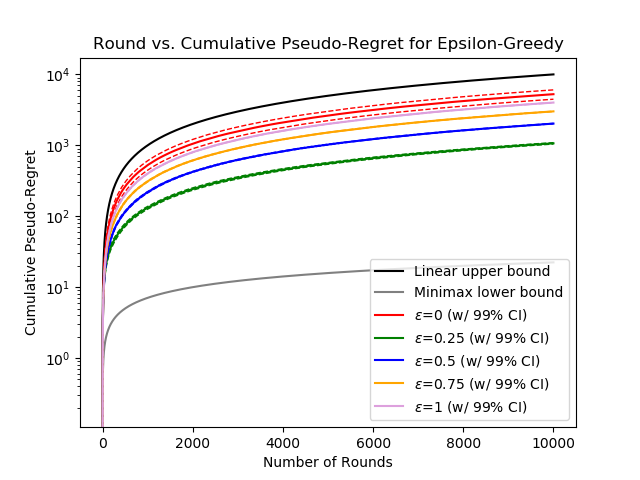
\includegraphics[width=\linewidth, height=0.75\linewidth]{epsilon-greedy.png}
\end{minipage}
\begin{minipage}[h]{0.5\linewidth}
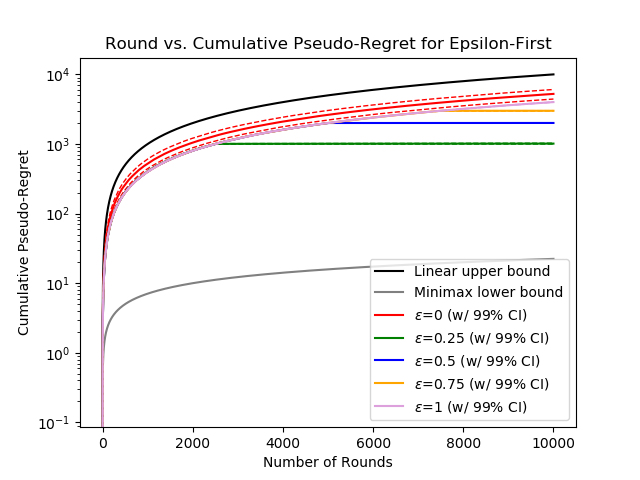
\includegraphics[width=\linewidth, height=0.75\linewidth]{epsilon-first.png}
\end{minipage}
\begin{minipage}[h]{0.5\linewidth}
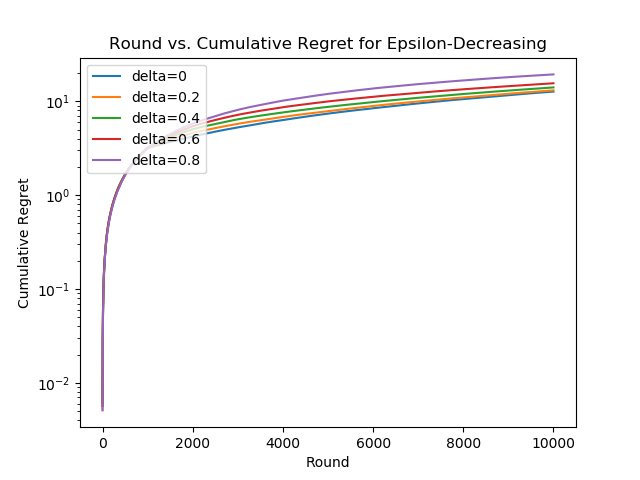
\includegraphics[width=\linewidth, height=0.75\linewidth]{epsilon-decreasing.png}
\end{minipage}
\begin{minipage}[h]{0.5\linewidth}
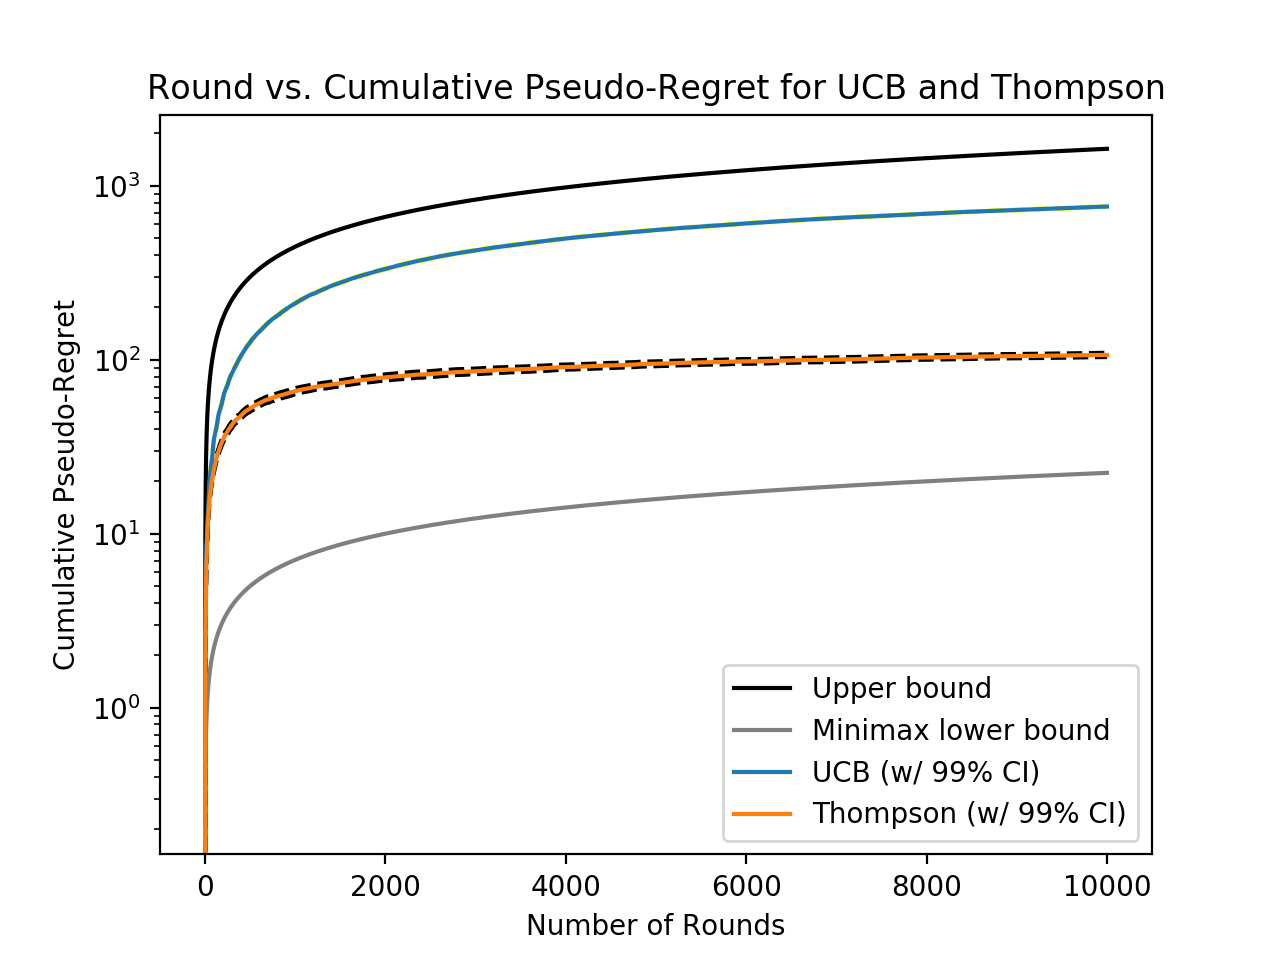
\includegraphics[width=\linewidth, height=0.75\linewidth]{ucb_thompson_stochastic.png}
\end{minipage}
\begin{minipage}[h]{0.5\linewidth}
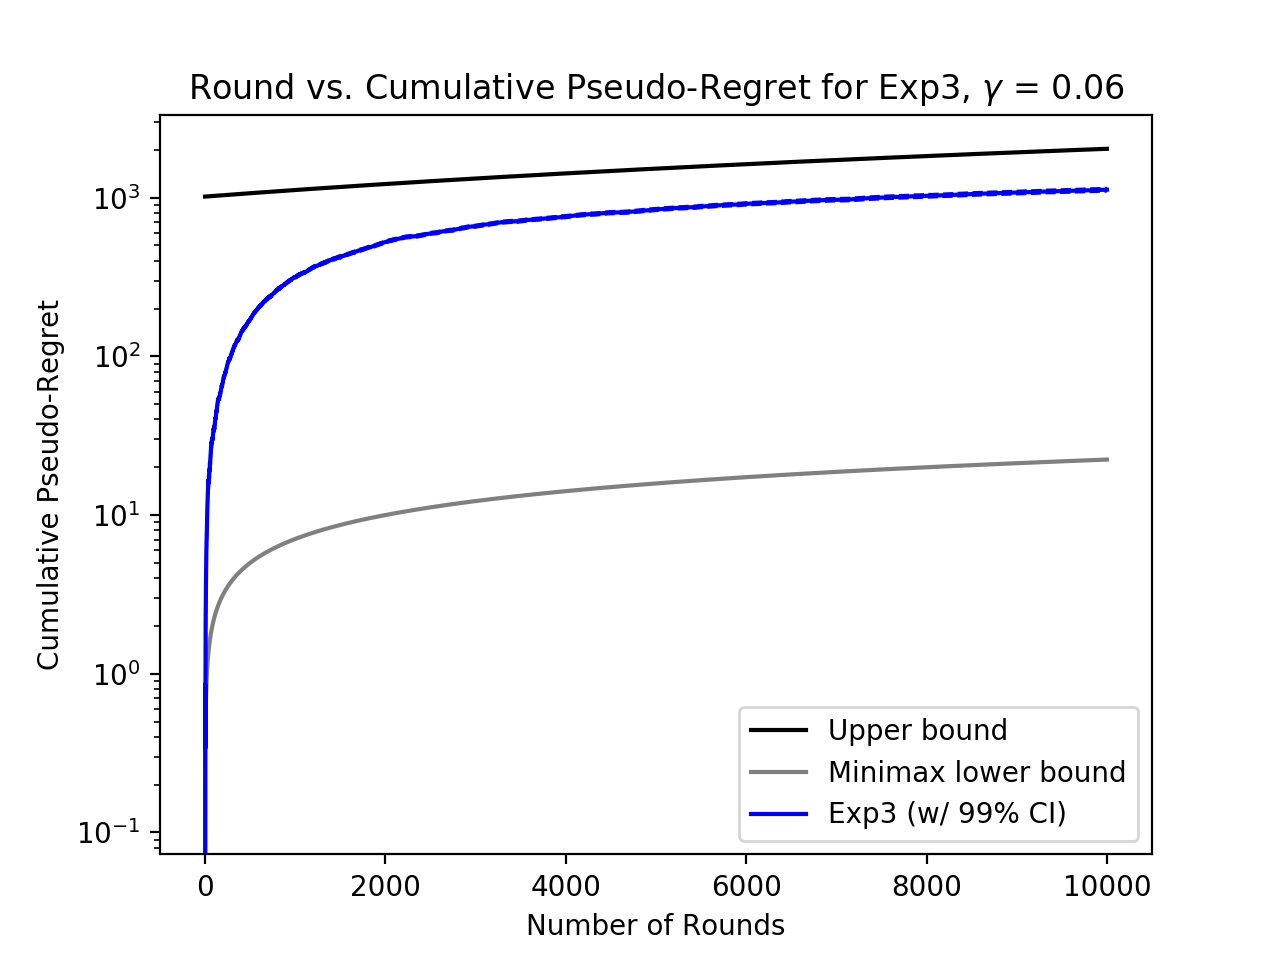
\includegraphics[width=\linewidth, height=0.75\linewidth]{exp3-2.png}
\end{minipage}
\begin{minipage}[h]{0.5\linewidth}
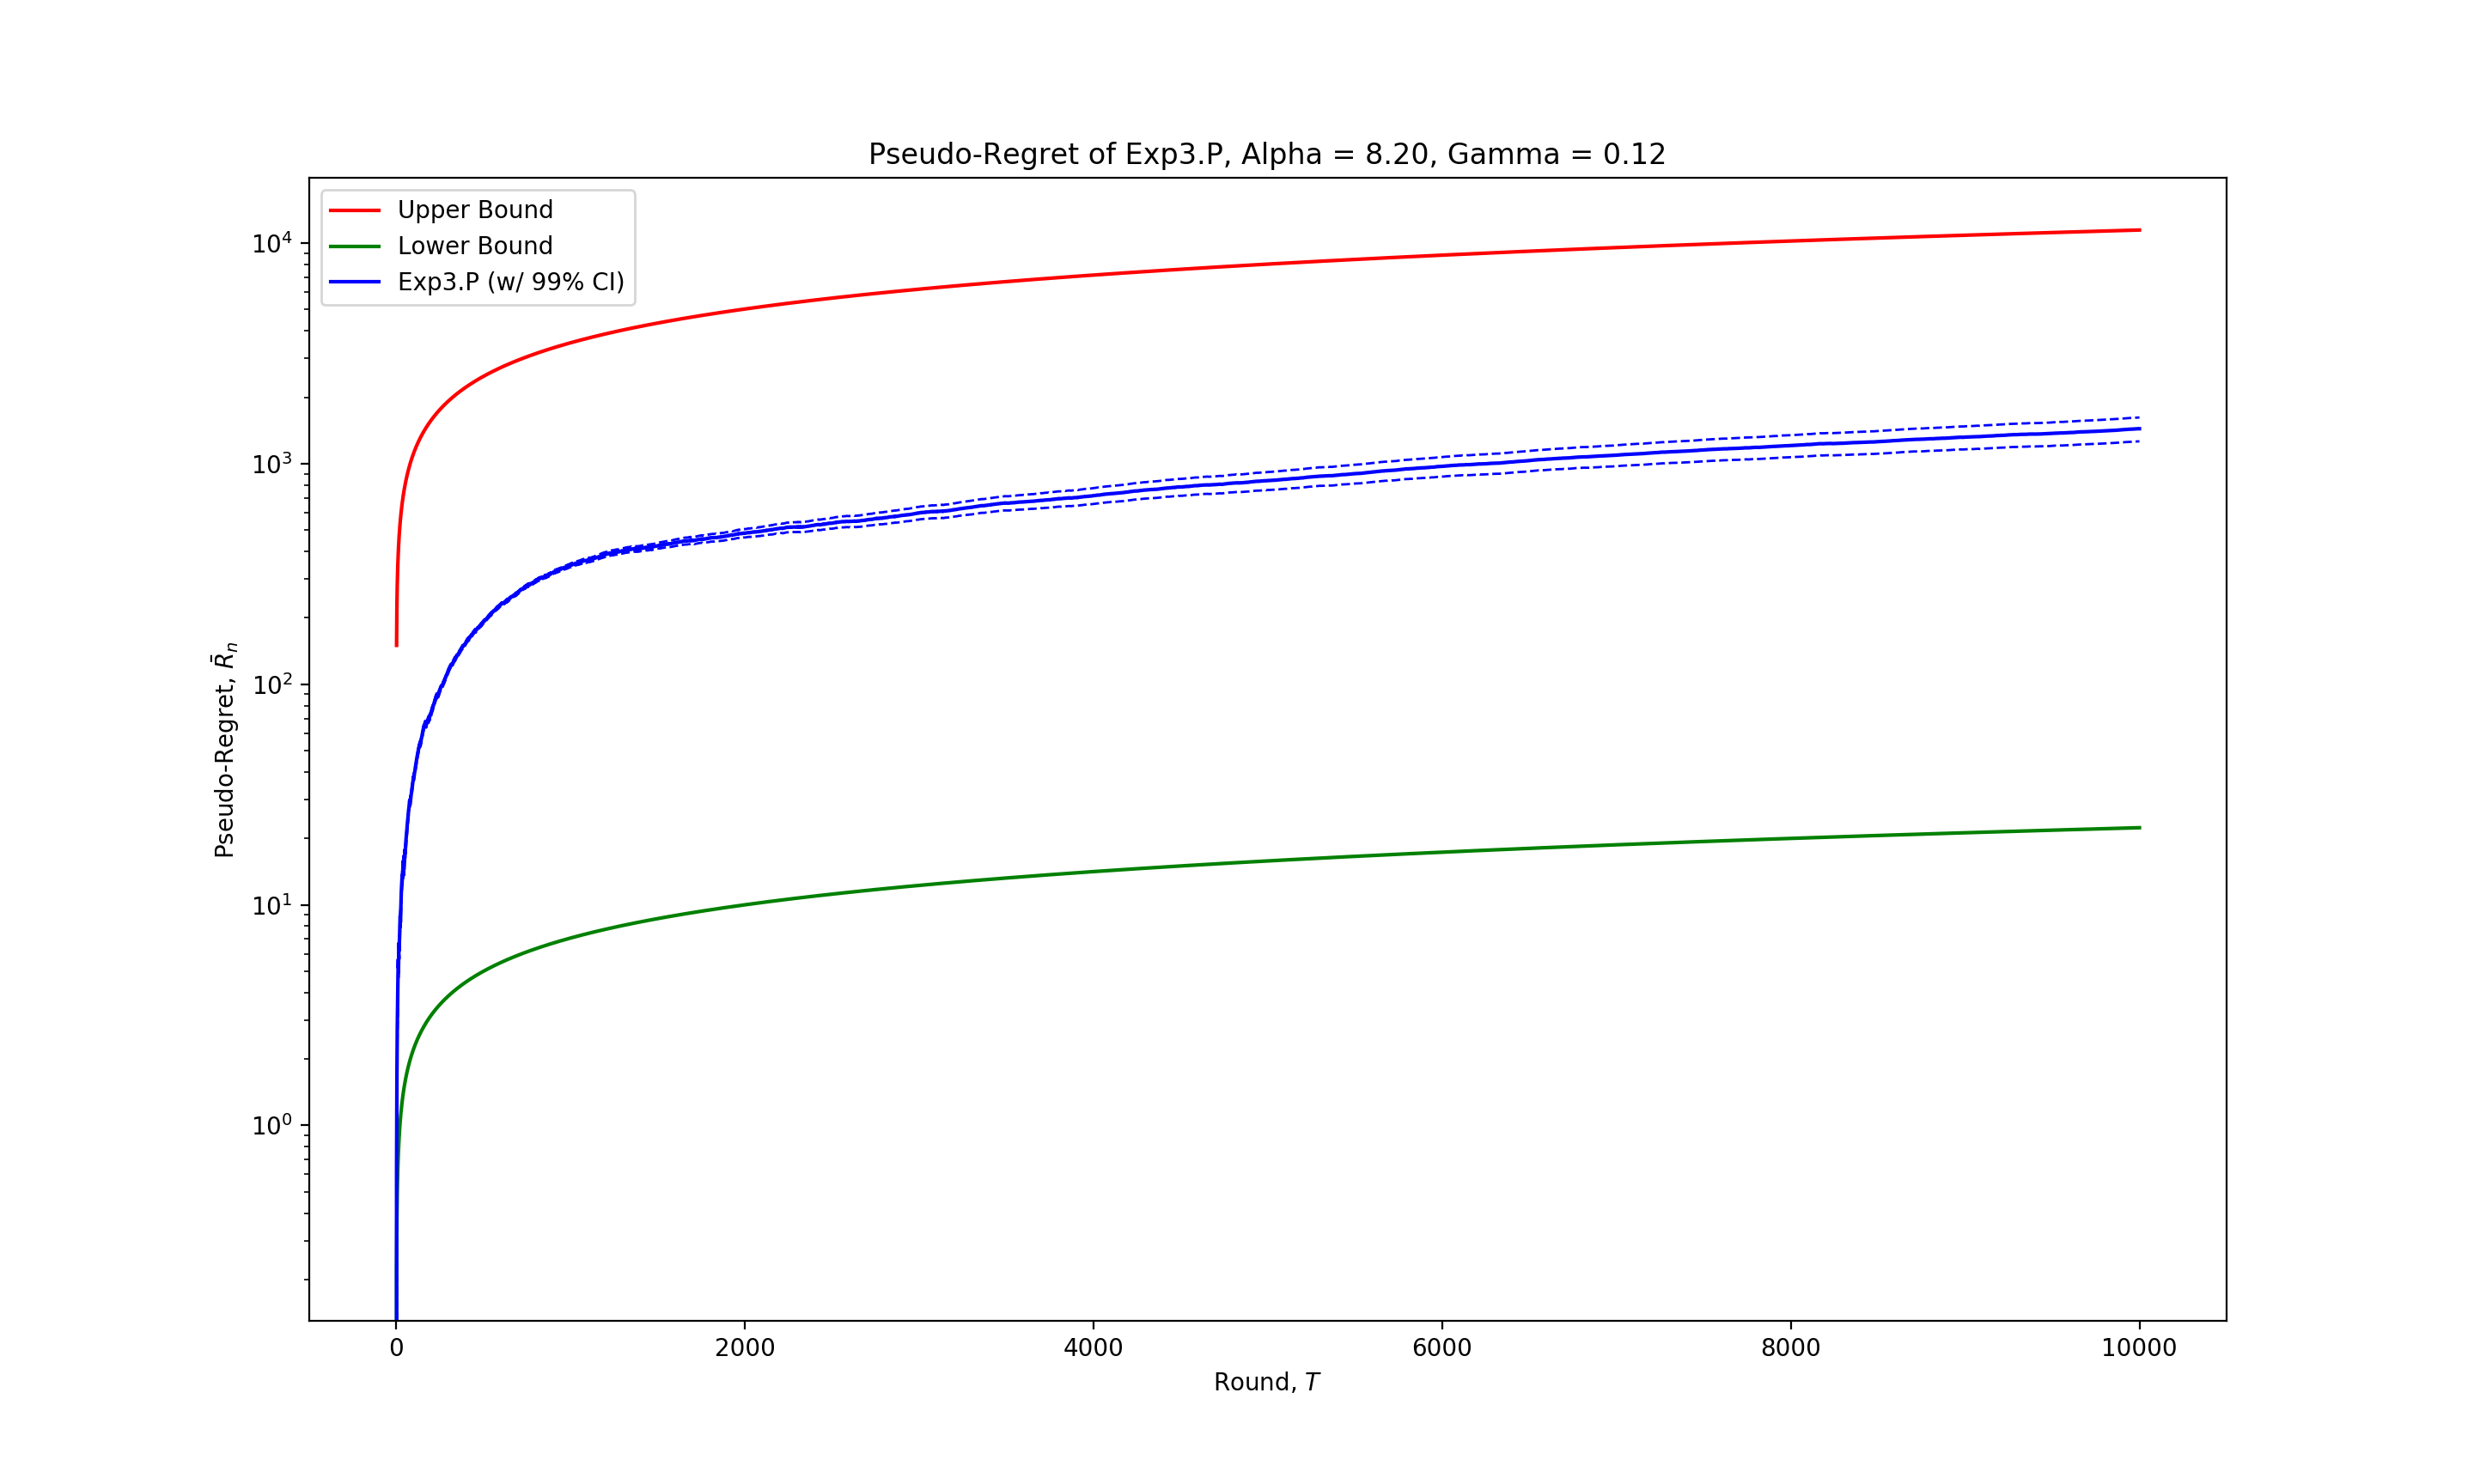
\includegraphics[width=\linewidth, height=0.75\linewidth]{exp3P-2.png}
\end{minipage}
\captionsetup{justification=centering}
\caption{Round vs. Cumulative Pseudo-Regret for Bandit Strategies}
\label{fig:stochastic-rewards-2}
\end{figure}

The Exp3 and Exp3.P algorithms, unsurprisingly, perform poorly because they do not assume stochastic i.i.d rewards and thus adopt a \textit{pessimistic} approach to the tradeoff between exploration and exploitation; that is, they insist on a high degree of exploration. The two strategies also experience high variance, again due to a constant amount of exploration (by construction) even though the underyling distributions are ``well-behaved" in the stochastic rewards setting. It should be noted, however, that the Exp3.P algorithm exhibits drastically higher variance that the Exp3 algorithm despite it purportedly controlling variance by design. This anomalous result is not well understood thus far.

Figure \ref{fig:stochastic-rewards-2} experimentally verifies the regret bounds of all strategies on Bernouilli trials. Clearly, each algorithm falls between its theoretical upper and lower bounds as expected. With that said, the upper and lower bounds are not tight. This highlights the fact that theory often provides good qualitative information about algorithms but not good quantitative information. Furthermore, the epsilon strategies are illuminating in that, empirically, low exploration rates (via $\epsilon$) are preferable. This makes sense, intuitively, since relatively few arms $K=20$ are considered and so the need for exploration is not high.

\subsubsection{Adversarial Rewards Setting}

\begin{figure}[H]
\scalemath{0.75}{
\begin{tabular}{|M{10cm}|M{5cm}|M{5cm}|}
\hline\textbf{Bandit Strategy} & \textbf{Mean $\bar{R}_{T}$} & \textbf{Variance $\bar{R}_{T}$} \\
\hline\textbf{UCB Algorithm} & 5,000.00 & 0.00 \\
\hline\textbf{Thompson Sampling} & 28.81 & 2,038.80 \\
\hline\textbf{Exp3 Algorithm, $\gamma=0.01$} & 29.70 & 2,301.61 \\
\hline\textbf{Exp3.P Algorithm, $\alpha=7.62$, $\gamma=0.00$} & 10.5 & 1,782.25 \\
\hline\textbf{Random Baseline} & -0.88 & 2,102.28 \\
\hline
\end{tabular}}
\captionsetup{justification=centering}
\caption{Mean and Variance of Pseudo-Regret after $T=10,000$ Rounds}
\label{fig:adversarial-rewards-1}
\end{figure}

Figure \ref{fig:adversarial-rewards-1} compares five of our multi-armed bandit algorithms in the adversarial setting. Note that Thompson sampling, Exp3 algorithm, Exp3.P Algorithm, and the random baseline algorithm all perform very well, while the UCB algorithm performs extremely poorly. The UCB algorithm's poor performance is not surprising. If it obtains good reward by choosing an action, it is more likely to choose the same action again. If it obtains poor reward by choosing an action, it is more likely to switch to another action. The adversary's behavior guarantees that the UCB algorithm will choose the worst outcome during each round. 

Thompson sampling performs well because the adversary's action is very predictable given the player's past reward and Bayesian inference can very well capture the pattern of reward given out by the adversary. Therefore, Thompson sampling has very good performance. The random algorithm performs well because in order for the adversary to successfully attack an algorithm, the adversary needs to be able to accurately predict an algorithm's subsequent actions given the algorithm's previous choices and rewards. With a random algorithm, it is impossible to predict what the algorithm will choose in the subsequent rounds, thus making it difficult to attack the random algorithm. The Exp3 and Exp3.P algorithms perform well because they are explicitly designed with the adversarial setting in mind and therefore approach exploration and exploitation pessimistically.

\begin{figure}[H]
\begin{minipage}[h]{0.5\linewidth}
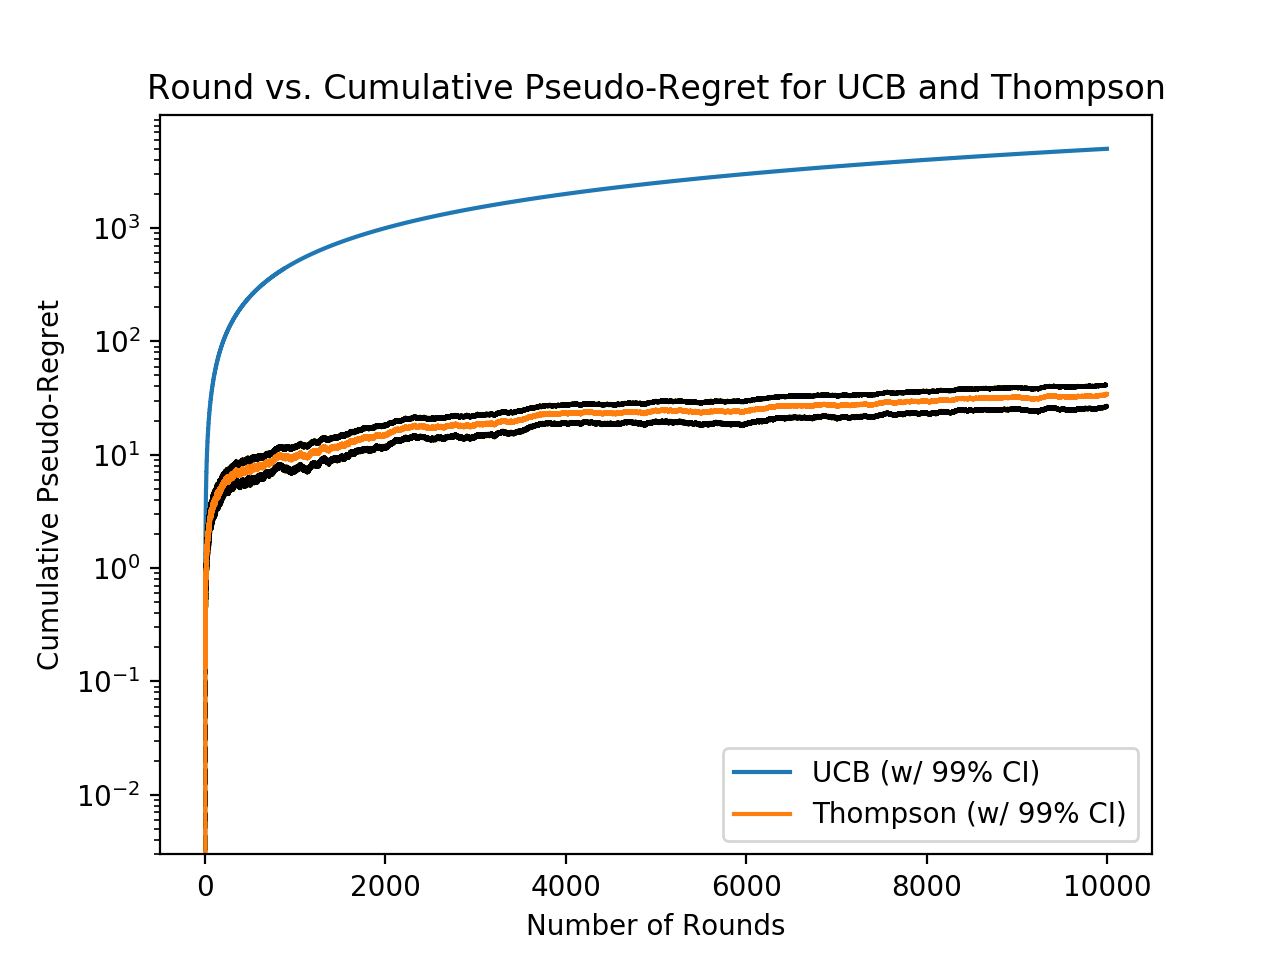
\includegraphics[width=\linewidth, height=0.75\linewidth]{ucb_thompson_adversarial.png}
\end{minipage}
\begin{minipage}[h]{0.5\linewidth}
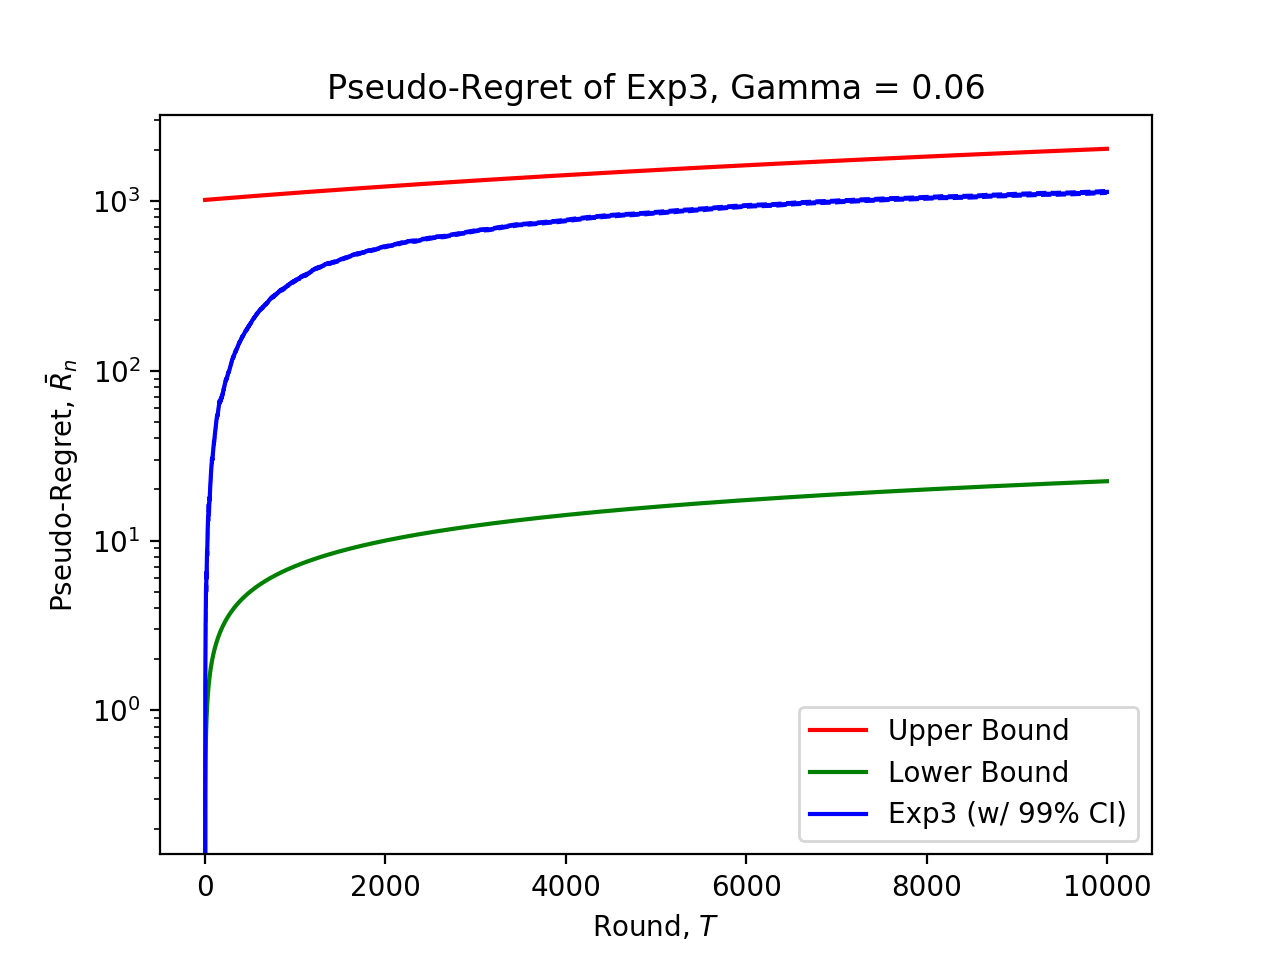
\includegraphics[width=\linewidth, height=0.75\linewidth]{exp3-1.png}
\end{minipage}
\begin{center}\begin{minipage}[h]{0.5\linewidth}
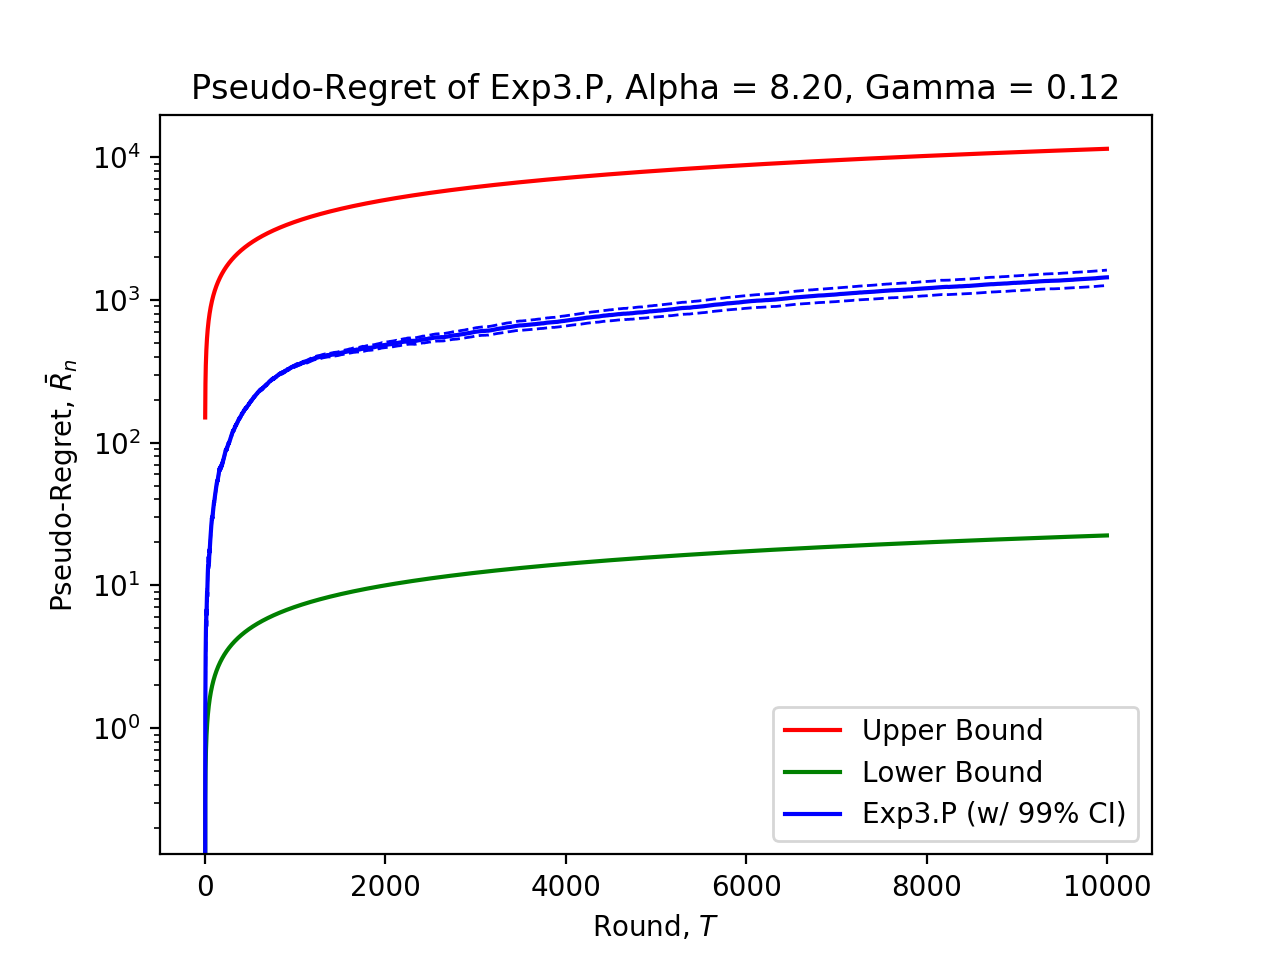
\includegraphics[width=\linewidth, height=0.75\linewidth]{exp3P-1.png}
\end{minipage}\end{center}
\captionsetup{justification=centering}
\caption{Round vs. Cumulative Pseudo-Regret for Bandit Strategies}
\label{fig:adversarial-rewards-2}
\end{figure}

\section{Conclusion}

Theory provides good qualitative guidance for practice. For example, an algorithm that assumes stochastic iid rewards, such as UCB, performs poorly in an adversarial setting and an algorithm that assumes adversarial rewards does not do well in the stochastic setting. When applying algorithms to the real world, we can choose algorithms based on whether the real world setting resembles the stochastic iid setting more closely or the real world setting resembles adversarial setting more closely. That said, theory does not provide very good quantitative guidance for practice. For example, although the performances of algorithms all fall between the theoretical lower bound and theoretical upper bound, these bounds are so loose that they do not provide any meaningful quantitative information.

\newpage
\printbibliography

\end{document}